\begin{document}
\maketitle

\begin{frame}
  \titlepage
\end{frame}

\cleardoublepage

\tableofcontents

\cleardoublepage

\section{Introduction}

\begin{frame}{DBIx::Class Training}
\note{
  Explain how I ended up doing DBIx::Class training.
}
\begin{figure}[!ht]
\centering
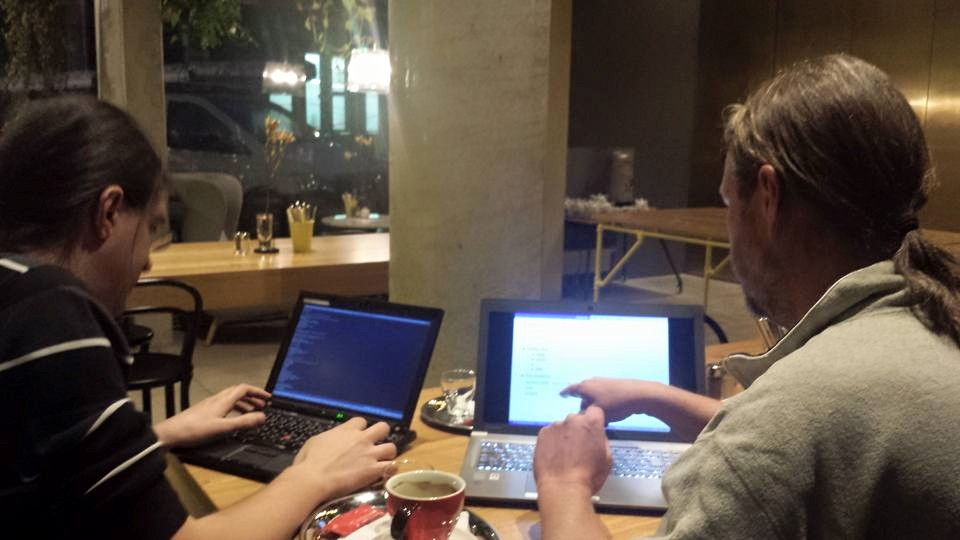
\includegraphics[width=1\linewidth]{img/training-preps.jpg}
\end{figure}
\end{frame}

\subsection{Best Thing Since Sliced Bread}

\begin{frame}{Best Thing Since Sliced Bread}

% https://en.wikipedia.org/wiki/Sliced_bread#/media/File:Brood.jpg

\begin{figure}[!ht]
\centering
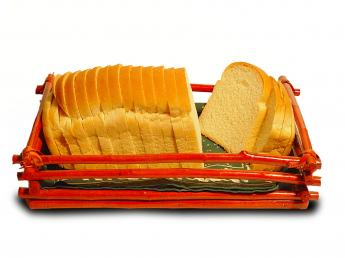
\includegraphics[width=1\linewidth]{img/sliced-bread.jpg}
\end{figure}
\end{frame}

\begin{frame}{Best Thing Since Sliced Bread}
\begin{itemize}
\item OO instead of SQL
\item Business Logic
\item Composability
\item Performance
\end{itemize}
\end{frame}

\subsection{Can of Worms}

\begin{frame}{Can of Worms}
\begin{figure}[!ht]
\centering

\includegraphics[width=0.75\linewidth]{img/canofworms.png}
\end{figure}
\end{frame}

\begin{frame}{Can of Worms}
\begin{itemize}
\item SQL::Abstract
\item Class names (Result, ResultSet)
\end{itemize}
\end{frame}

\subsection{DBIx::Class instead of SQL queries}

\begin{frame}{SQL is ...}
\begin{itemize}
\item SQL is ... boring
\item SQL is ... complex
\item SQL is ... governed by "15 competing standards"
\item SQL is ... not object oriented
\end{itemize}
\end{frame}


Using DBIx::Class allows you move all your business logic
into the database schema instead scattering it around a (web)
application.

\subsection{Business Logic}
\begin{frame}{Business Logic}
% move business logic into schema
% https://pixabay.com/en/gear-gears-euro-forex-dollar-384743/
\begin{figure}[!ht]
\centering

\includegraphics[width=0.75\linewidth]{img/business-logic.jpg}
\end{figure}
\end{frame}

\begin{frame}{Business Logic Benefits}
\begin{itemize}
\item Multiple Consumers
\begin{itemize}
\item Web application(s)
\item Cron jobs, scripts
\item Test environments
\end{itemize}
\item Changes / DRY
\end{itemize}
\end{frame}

\subsection{Performance}

All the experience, tests and different areas in which 
DBIx::Class is applied makes it perform better than
handwritten SQL is most cases.

\begin{frame}{Performance}
\begin{itemize}
\item Experience
\item Test results
\item Use cases
\end{itemize}
\end{frame}
 
In case you feel that isn't correct, please call our hotline:

\begin{frame}
\begin{figure}[!ht]
\centering
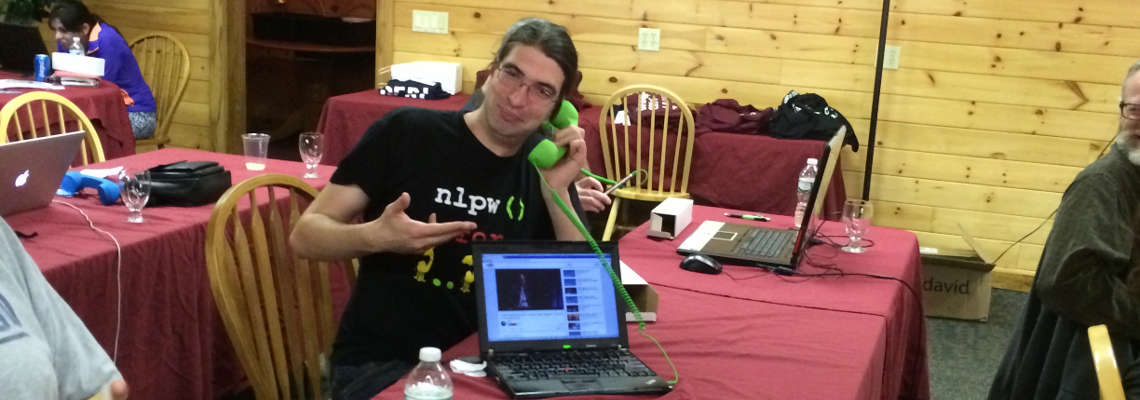
\includegraphics[width=1\linewidth]{img/perldance-2014-modern-tech.jpg}
\end{figure}
\end{frame}

But if you want to resort to SQL at some point, DBIx::Class allows you
to that too

\begin{frame}[fragile]{Literal SQL}
\begin{lstlisting}
$schema->resultset('PlaceVisited')->search(
{
  users_id => {
    -in => \[
       'SELECT users_id FROM users WHERE users_id > ?',
       2
    ]
  }
});
\end{lstlisting}
\end{frame}

But please don't complain if that leads to headache
and wasted time better spent on proper DBIx::Class
code.

\begin{frame}{SQL Headache}
% https://pixabay.com/en/stress-man-hand-flame-burn-fire-864141/
\begin{figure}[!ht]
\centering

\includegraphics[width=1\linewidth]{img/stress.jpg}
\end{figure}
\end{frame}

\section{Other Nice Stuff}
\subsection{Subclassing Schema}

You can also subclass schemas.

* add new columns to existing tables

\begin{frame}[fragile]{Subclass Example}
\begin{lstlisting}
package PerlDance::Schema;

use base 'Interchange6::Schema';

Interchange6::Schema->load_namespaces(
    default_resultset_class => 'ResultSet',
    result_namespace        =>
        [ 'Result', '+PerlDance::Schema::Result' ],
    resultset_namespace     =>
        [ 'ResultSet', '+PerlDance::Schema::ResultSet' ],
);
\end{lstlisting}
\end{frame}

\section{Composability}

Composability means that you don't need to construct the
complete at once, but compose it together, e.g with
chaining.

The underlying mechanism is that \verb|->search| on a
ResultSet actually doesn't search.


\subsection{Starting with DBIx::Class}

\begin{frame}{Starting with DBIx::Class}
\begin{itemize}
\item Existing project
\item New project
\end{itemize}
\end{frame}

\subsubsection{Existing Project}

You can use \verb|dbicdump| to create a ``boilerplate'' schema from the
existing database.

\begin{frame}[fragile]{dbicdump}
\begin{lstlisting}
dbicdump -o dump_directory=/home/dance/TravelDance/lib 
         TravelDance::Schema 
         dbi:Pg:dbname=perldance
\end{lstlisting}
\end{frame}

\subsubsection{New Project}

For new projects we recommend to write the schema first.

\begin{frame}[fragile]{New Project}
Write Schema first
\end{frame}


\subsection{DBIC Classes}

\begin{frame}{DBIC Classes}
\begin{itemize}
\item One \emph{schema} class
\begin{itemize}
\item TravelDance::Schema
\end{itemize}
\item One \emph{result} class for each source ( table, view, SQL fragment, etc )
\begin{itemize}
\item TravelDance::Schema::Result::Country
\item TravelDance::Schema::Result::PlaceVisited
\item TravelDance::Schema::Result::User
\end{itemize}
\item One \emph{result set} class for each source ( table, view, SQL fragment, etc )
\begin{itemize}
\item TravelDance::Schema::ResultSet::Country
\item TravelDance::Schema::ResultSet::PlaceVisited
\item TravelDance::Schema::ResultSet::User
\end{itemize}
\end{itemize}
\end{frame}

\subsubsection{Schema Class}

Here we see the minimal DBIx::Class schema definition:

\begin{frame}[fragile]{Schema Class}
\begin{lstlisting}
package TravelDance::Schema;
use warnings;
use strict;
use base 'DBIx::Class::Schema';

__PACKAGE__->load_namespaces();
1;
\end{lstlisting}
\end{frame}

\verb|load_namespaces| searches \verb|TravelDance::Schema::Result{Set}::*|
for Result and ResultSet classes and loads them into the schema.

\subsubsection{Result Classes}

\begin{frame}{Result Classes}
\begin{itemize}
\item Need one result class for each table
\item Country => countries
\item PlaceVisited => places\_visited
\item User => users
\end{itemize}
\end{frame}

\subsubsection{Result Class Definition}
Describes each result class and the database table behind it. 

See \href{https://metacpan.org/pod/DBIx::Class::ResultSource}{DBIx::Class::ResultSource} for more details.

\begin{frame}{Result Class Definition}

\begin{itemize}
\item Source (RDBMS-side) name
\item Columns
\item Primary key
\item Relationships
\end{itemize}
\end{frame}

\subsubsection{Vanilla DBIC Result Class}

\begin{frame}[fragile]{Vanilla DBIC Result Class for Country I}
\begin{lstlisting}
package TravelDance::Schema::Result::Country;
use warnings;
use strict;
use base 'DBIx::Class::Core';

__PACKAGE__->table('countries');

__PACKAGE__->add_columns(
    country_iso_code => {
        data_type => "char",
        size      => 2,
    },
    name => {
        data_type => "varchar",
        size      => 255,
    },
);
\end{lstlisting}
\textit{... to be continued.}
\end{frame}

\begin{frame}[fragile]{Vanilla DBIC Result Class for Country II}
\begin{lstlisting}
__PACKAGE__->set_primary_key("country_iso_code");

__PACKAGE__->has_many(
    places_visited =>
      "TravelDance::Schema::Result::PlaceVisited",
      'country_iso_code'
);

__PACKAGE__->many_to_many(
    users => "places_visited", "user"
);

1;
\end{lstlisting}
\end{frame}

\subsubsection{Candy DBIC Result Class}

\begin{frame}[fragile]{Candy DBIC Result Class for Country I}
\begin{lstlisting}
package TravelDance::Schema::Result::Country;
use TravelDance::Schema::Candy;

primary_column country_iso_code => {
    data_type => "char",
    size      => 2
};

column name => {
    data_type => "varchar",
    size      => 255
};
\end{lstlisting}
\end{frame}

\begin{frame}[fragile]{Candy DBIC Result Class for Country II}
\begin{lstlisting}
has_many
  places_visited =>
  "TravelDance::Schema::Result::PlaceVisited",
  'country_iso_code';

many_to_many users => "places_visited", "user";
\end{lstlisting}
\end{frame}

\subsection{DBIx::Class::Schema::Config}

\begin{frame}{DBIx::Class::Schema::Config}
\begin{itemize}
\item Credential Management for DBIx::Class.
\item Move DSN, username, password out of code
\end{itemize}
\end{frame}

\subsubsection{Typical script for DBIx::Class}
\begin{frame}[fragile]{Typical script for DBIx::Class}
\begin{lstlisting}
use TravelDance::Schema;
my $dsn = 'dbi:SQLite:traveldance.db';
my %dbi_params = (
    on_connect_call            => 'use_foreign_keys',
    quote_names                => 1,
    sqlite_unicode             => 1,
    sqlite_see_if_its_a_number => 1,
);
my $schema = TravelDance::Schema->connect( $dsn,,, 
    \%dbi_params );
\end{lstlisting}
\end{frame}

Move the DBIC config to \textasciitilde/.dbic.yml:

\begin{frame}[fragile]{Configuration File \textasciitilde/.dbic.yml}
\begin{lstlisting}
traveldance:
  dsn: 'dbi:SQLite:traveldance.db'
  on_connect_call: 'use_foreign_keys'
  quote_names: 1
  sqlite_unicode: 1
  sqlite_see_if_its_a_number: 1
\end{lstlisting}
\end{frame}

Now we adjust the schema class and the script to use
the configuration file:

\begin{frame}[fragile]{Using the configuration file}
Change the base class of the Schema:

\begin{lstlisting}
package TravelDance::Schema;
use base 'DBIx::Class::Schema::Config';
\end{lstlisting}

Update the script:

\begin{lstlisting}
use TravelDance::Schema;
my $schema = TravelDance::Schema
   ->connect( 'traveldance' );
\end{lstlisting}
\end{frame}

Configuration format and files:

\begin{frame}[fragile]{Configuration format and files}
\begin{itemize}
\item Config::Any
\begin{itemize}
\item YAML
\item JSON
\item XML
\item ...
\end{itemize}
\item File locations
\begin{description}
\item[project] \verb|./dbic.*| \emph{without} dot
\item[user] \verb|~/.dbic.*| \emph{with} dot
\item[system-wide] \verb|/etc/dbic.*|
\end{description}
\end{itemize}
\end{frame}


\section{DBIx::Class Helpers}

\begin{frame}{DBIx::Class Helpers}
Simplify the common case stuff for DBIx::Class.
\end{frame}

\begin{frame}{DBIx::Class Helpers}
\begin{figure}[!ht]
\centering

\includegraphics[width=0.4\linewidth]{img/frew.png}
\caption{Arthur Axel "fREW" Schmidt}
\end{figure}
\end{frame}

\subsection{CorrelateRelationship}

\begin{frame}{CorrelateRelationship}

Problem: we want a count of rows in a related table

\end{frame}

So the obvious approach for this is:

\begin{frame}[fragile]{CorrelateRelationship}
\begin{lstlisting}
    my $rs = $schema->resultset('Author')->search(
        undef,
        {
            join       => 'books',
            '+columns' => {
                book_count => {
                    count => 'books.id'
                }
            },
            distinct   => 1,    # let DBIC work out group_by for us
        }
    );
\end{lstlisting}
\end{frame}
This causes a number of problems:

\begin{itemize}
\item Depending on engine, COUNT’s that aren’t COUNT(*) tend to be slow as
they do table scans.
\item This is hard to chain since we've introduced JOIN and GROUP BY and
collapsed COUNTs might produced unexpected results.
\item We cannot add other interesting data from the places\_visited in the same query (such as date of most recent visit).
\end{itemize}

\begin{frame}[fragile]{CorrelateRelationship}
\begin{lstlisting}
Much nicer to do:

    package MyApp::Schema::ResultSet::Author;

    use parent 'DBIx::Class::ResultSet';

   
__PACKAGE__->load_components(qw(Helper::ResultSet::CorrelateRelationship));

    sub with_book_count {
        my $self = shift;

        $self->search(
            undef,
            {
                '+columns' => {
                    book_count =>
$self->correlate('books')->count_rs->as_query
                }
            }
        );
    }
\end{lstlisting}
\end{frame}

\begin{frame}[fragile]{CorrelateRelationship}
Then elsewhere:

\begin{lstlisting}
my $rs = $schema->resultset('Author')->with_book_count;

The SQL query will look something like this:

  SELECT me.id, me.name, me.foo, ..., (
    SELECT COUNT( * )
      FROM books books_alias
     WHERE books_alias.id = authors.id
   )
  FROM authors me

This is *much* faster and *always* chainable since no JOIN, GROUP BY, or
other junk added to query.
\end{lstlisting}
\end{frame}

Cool example from Interchange6::Schema::ResultSet::Product :

\begin{lstlisting}
    sub with_average_rating {
        my $self = shift;

        return $self->search(
            undef,
            {
                '+select' => [
                    {
                        coalesce => [

                            $self->correlate('canonical')
                              ->related_resultset('_product_reviews')
                              ->search_related(
                                'message',
                                { 'message.approved' => 1,
'message.public' => 1 }
                             
)->get_column('rating')->func_rs('avg')->as_query,

                            $self->correlate('_product_reviews')
                              ->search_related(
                                'message',
                                { 'message.approved' => 1,
'message.public' => 1 }
                             
)->get_column('rating')->func_rs('avg')->as_query,

                          ],
                        -as => 'average_rating'
                    }
                ],
                '+as' => ['average_rating'],
            }
        );
    }
\end{lstlisting}

\subsection{Helper::Resultset::Me}

Predefined queries present a problem: what is the table alias I need to use?
We can do:

\begin{frame}[fragile]{Helper::Resultset::Me}
\begin{lstlisting}
sub in_germany {
    my $self = shift;
    my $current_source_alias =
        $self->current_source_alias;
    return $self->search(
        { "$current_source_alias.country_iso_code"
          => 'DE' }
    );
}
\end{lstlisting}
\end{frame}

but using this helper makes things much simpler:

\begin{frame}[fragile]{Helper::Resultset::Me}
\begin{lstlisting}
sub in_germany {
    my $self = shift;


    return $self->search(
        { $self->me('country_iso_code') => 'DE' }
    );

}
\end{lstlisting}
\end{frame}

\subsection{Helper::Resultset::Random}

We use this in Interchange6 for finding random 'similar products' and other
such searches.

Three random countries:

\begin{frame}[fragile]{Helper::Resultset::Me}
\begin{lstlisting}

my $countries = $schema->resultset('Country')->rand(3);

\end{lstlisting}
\end{frame}

\subsection{Helper::ResultSet::RemoveColumns}
Have a result class with a large number of columns and you want all except
one (or more) of them:

\begin{frame}[fragile]{Helper::ResultSet::RemoveColumns}
\begin{lstlisting}
my $rs = $schema->resultset('User')->search(
    undef,
    {
        remove_columns => [ 'password' ],
    }
);
\end{lstlisting}
\end{frame}

Make that the default for searches (though this is not generally recommended):

\begin{frame}[fragile]{Helper::ResultSet::RemoveColumns}
\begin{lstlisting}
package TravelDance::Schema::Result::User;

__PACKAGE__->resultset_attributes(
    { remove_columns => [ 'password' ] }
);
\end{lstlisting}
\end{frame}

\subsection{Helper::ResultSet::Shortcut}

\begin{frame}[fragile]{distinct Shortcut}

\verb|distinct| shortcut:

\begin{lstlisting}
$rs->distinct;
\end{lstlisting}

equivalent to:

\begin{lstlisting}
$rs->search(undef, { distinct => 1 });
\end{lstlisting}
\end{frame}

\begin{frame}[fragile]{group\_by Shortcut}

\verb|group_by| shortcut:

\begin{lstlisting}
$rs->group_by([ qw/ some column names / ]);
\end{lstlisting}

equivalent to:

\begin{lstlisting}
$rs->search(undef, { 
    group_by([ qw/ some column names / ] 
});
\end{lstlisting}
\end{frame}

\begin{frame}[fragile]{order\_by Shortcut}

\verb|order_by| Shortcut:

\begin{lstlisting}
$rs->order_by({ -desc => 'col1' });
\end{lstlisting}

equivalent to:

\begin{lstlisting}
$rs->search(undef, { order_by => { -desc => 'col1' });
\end{lstlisting}

\end{frame}

\begin{frame}[fragile]{order\_by Shortcut}

Funky magic stuff:
\begin{lstlisting}
$rs->order_by('!col1')
# { order_by => { -desc => 'col1' } }

$rs->order_by('col1,col2')
# { order_by => [{ -asc => 'col1' },{ -asc => 'col2' }]}

$rs->order_by('col1,!col2')
# { order_by => [{ -asc => 'col1' },{ -desc => 'col2' }]}
\end{lstlisting}
\end{frame}

\begin{frame}[fragile]{hri Shortcut}

\verb|hri| shortcut:

\begin{lstlisting}
$rs->hri;
\end{lstlisting}

equivalent to:

\begin{lstlisting}
$rs->search( undef, {
    result_class => 
        'DBIx::Class::ResultClass::HashRefInflator'
});
\end{lstlisting}
\end{frame}

\begin{frame}[fragile]{page Shortcut}

\verb|page| shortcut:

\begin{lstlisting}
$rs->page(2);
\end{lstlisting}

equivalent to:

\begin{lstlisting}
$rs->search( undef, { page => 2 } );
\end{lstlisting}

\end{frame}

rows / limit

\begin{frame}[fragile]{rows / limit Shortcut}

\begin{lstlisting}
$rs->rows(3);
\end{lstlisting}

or:

\begin{lstlisting}
$rs->limit(3);
\end{lstlisting}

equivalent to:

\begin{lstlisting}
$rs->search( undef, { rows => 3 } );
\end{lstlisting}

\end{frame}

\begin{frame}[fragile]{limited\_page Shortcut}

\verb|limited_page| shortcut:

\begin{lstlisting}
$rs->limited_page( 2, 3 );
\end{lstlisting}

equivalent to:

\begin{lstlisting}
$rs->search( undef, { page => 2, rows => 3 } );
\end{lstlisting}

\end{frame}

\begin{frame}[fragile]{has\_rows Shortcut}

A lighter way to check if the resultset has data compared to using count.

\begin{lstlisting}
$rs->has_rows;
\end{lstlisting}

equivalent to:

\begin{lstlisting}
$rs->search( undef, { rows => 1 } )->next;
\end{lstlisting}
\end{frame}

results\_exists:

\begin{frame}[fragile]{results\_exists Shortcut}

An alternative way to check if the resultset has data using the EXISTS SQL function. Possibly lighter-weight than using count.

\begin{lstlisting}
$rs->search(...)->results_exist
\end{lstlisting}
\end{frame}

\begin{frame}[fragile]{columns Shortcut}

\verb|columns| shortcut:

\begin{lstlisting}
$rs->columns([qw/ first_name last_name /]);
\end{lstlisting}

equivalent to:

\begin{lstlisting}
$rs->search( undef, { 
    columns => [qw/ first_name last_name /] 
} );
\end{lstlisting}

\end{frame}

\begin{frame}[fragile]{add\_columns Shortcut}

\verb|add_columns| shortcut:

\begin{lstlisting}
$rs->add_columns([qw/ some column names /]);
\end{lstlisting}

equivalent to:

\begin{lstlisting}
$rs->search( undef,
    { '+columns' => [qw/ some columns names /] }
);
\end{lstlisting}
\end{frame}

\begin{frame}[fragile]{prefetch Shortcut}

\verb|prefetch| shortcut:

\begin{lstlisting}
$rs->prefetch( { places_visited => 'country' } );
\end{lstlisting}

equivalent to:

\begin{lstlisting}
$rs->search( undef, { 
    prefetch => { places_visited => 'country' } 
} );
\end{lstlisting}

\end{frame}

% null ( @columns || \@columns )

\begin{frame}[fragile]{null Shortcut}

\verb|null| shortcut:

\begin{lstlisting}
$rs->null( 'col1', 'col2' );
\end{lstlisting}

or:

\begin{lstlisting}
$rs->null([ 'col1', 'col2' ]);
\end{lstlisting}

equivalent to:

\begin{lstlisting}
$rs->search({ col1 => undef, col2 => undef });
\end{lstlisting}
\end{frame}

%not\_null ( @columns || \@columns )

\begin{frame}[fragile]{not\_null Shortcut}

\verb|not_null| shortcut:

\begin{lstlisting}
$rs->not_null( 'col1', 'col2' );
\end{lstlisting}

or:

\begin{lstlisting}
$rs->not_null([ 'col1', 'col2' ]);
\end{lstlisting}

equivalent to:

\begin{lstlisting}
$rs->search({
    col1 => { '!=' => undef }, col2 => { '!=' => undef }
});
\end{lstlisting}
\end{frame}

%like ( @columns || \@columns, $cond )

\begin{frame}[fragile]{like Shortcut}

\verb|like| shortcut:

\begin{lstlisting}
$rs->like( 'city', 'region', '%York' );
\end{lstlisting}

or:

\begin{lstlisting}
$rs->like([ 'city', 'region' ], '%York' );
\end{lstlisting}

equivalent to:

\begin{lstlisting}
$rs->search(
    { city => { -like => '%York' },
    { region => { -like => '%York' },
);
\end{lstlisting}
\end{frame}

% not\_like ( @columns || \@columns, $cond )

\begin{frame}[fragile]{not\_like Shortcut}

\verb|not_like| shortcut:

\begin{lstlisting}
$rs->not_like( 'city', 'region', '%York' );
\end{lstlisting}

or:

\begin{lstlisting}
$rs->not_like([ 'city', 'region' ], '%York' );
\end{lstlisting}

equivalent to:

\begin{lstlisting}
$rs->search(
    { city => { -not_like => '%York' },
    { region => { -not_like => '%York' },
);

\end{lstlisting}
\end{frame}

\subsection{Helper::Row::NumifyGet}

\begin{frame}[fragile]{Helper::Row::NumifyGet}

Force numeric context on numeric columns:

\begin{lstlisting}
package TravelDance::Schema::Result::Foo_Bar;

use TravelDance::Schema::Candy -components =>
    [qw(Helper::Row::NumifyGet)];

column foo => {
    data_type   => 'integer',
    is_nullable => 0,
    is_numeric  => 1,   # the magic key
};
\end{lstlisting}
\end{frame}

\begin{frame}[fragile]{Helper::Row::NumifyGet}
\begin{lstlisting}
sub TO_JSON {
    return {
        # 0 instead of "0" due to context
        foo => $self->foo,  
    }
}
\end{lstlisting}
\end{frame}

\subsection{Helper::Row::OnColumnChange}

\begin{frame}[fragile]{Helper::Row::OnColumnChange}

Do things when the value of a column changes.

\begin{itemize}
\item before\_column\_change
\item around\_column\_change
\item after\_column\_change
\end{itemize}

\end{frame}

\begin{frame}[fragile]{Helper::Row::OnColumnChange}

\begin{lstlisting}
package TravelDance::Schema::Result::User;

use TravelDance::Schema::Candy -components =>
    [qw(Helper::Row::OnColumnChange 
        InflateColumn::DateTime)];

use DateTime;

column last_password_change => {
    data_type => timestamp,
};
\end{lstlisting}
\end{frame}

\begin{frame}[fragile]{Helper::Row::OnColumnChange}

On password change:

\begin{itemize}
\item check new password against old one
\item update \verb|last_password_change| column
\end{itemize}

\end{frame}

\begin{frame}[fragile]{Helper::Row::OnColumnChange}
\begin{lstlisting}
after_column_change password => {
    method   => 'change_password',
    txn_wrap => 1,  # wrap it all in a transaction
};
\end{lstlisting}
\end{frame}

\begin{frame}[fragile]{Helper::Row::OnColumnChange}
\begin{lstlisting}
sub change_password {
    my ( $self, $old_value, $new_value ) = @_;
    if ( $self->check_password($new_value) ) {
        $self->throw_exception("Password not changed")
    }
    else {
        $self->update(
            { last_password_change => DateTime->now() }
        );
    }
}
\end{lstlisting}
\end{frame}

\subsection{Helper::Schema::DateTime}

\begin{frame}[fragile]{Helper::Schema::DateTime}
VisitedPlaces visited in the last year:

\begin{lstlisting}
my $one_year_ago = $schema->format_datetime(
    DateTime->now->subtract( year => 1 )
);

my $rs = $schema->resultset('PlaceVisited')->search(
    {
        visited => { '>' => $one_year_ago }
    }
);
\end{lstlisting}
\end{frame}

\begin{frame}[fragile]{Helper::Schema::DateTime}

Without the helper:

\begin{lstlisting}
my $dtf = $schema->storage->datetime_parser; # boilerplate
my $one_year_ago = $dtf->format_datetime(
    DateTime->now->subtract( year => 1 )
);

my $rs = $schema->resultset('PlaceVisited')->search(
    {
        visited => { '>' => $one_year_ago }
    }
);
\end{lstlisting}
\end{frame}

\subsection{Helper::QuoteNames}

\begin{frame}{Helper::QuoteNames}
This should always be used. Force quote\_names in your database
connect\_info so nobody can forget to add it later.
\end{frame}

\subsection{HashRefInflator}

Using the HashRefInflator makes sense when you need to quickly retrieve
data from a massive resultset or you need a list of hash references anyway,
e.g. for input to a template in a web application.

\begin{frame}[fragile]{HashRefInflator}
\begin{lstlisting}
my $rs = $schema->resultset('Country')->search({}, {
   result_class
     => 'DBIx::Class::ResultClass::HashRefInflator',
 });
\end{lstlisting}
\end{frame}

\begin{frame}[fragile]{HashRefInflator with HRI helper}
\begin{lstlisting}
my $rs = $schema->resultset('Country')->search({})->hri;

# since 'search' here is redundant we can just use:
my $rs = $schema->resultset('Country')->hri;
\end{lstlisting}
\end{frame}

% \section{Writing Tests}
% \begin{frame}{Writing Tests}
% \end{frame}

\section{Deployment Handler}

\subsection{Deploy/Upgrade/Downgrade}

\begin{frame}{Deployment Handler}
\begin{itemize}
\item DBIx::Class::DeploymentHandler
\item Deploy databases
\item Upgrade databases
\item Downgrade databases
\end{itemize}
\end{frame}

\subsection{Principles}

\begin{frame}{Principles}
\begin{itemize}
\item Create backup
\item Change schema
\item Add custom scripts
\item Bump version number
\item Prepare upgrade
\item Deploy upgrade
\end{itemize}
\end{frame}

Note: create backup can be done by DeploymentHandler itself.

\subsection{Change Schema}

\begin{frame}{Change Schema}
\begin{itemize}
\item Add table
\item Add column
\item Alter column
\end{itemize}
\end{frame}

\subsection{Bump version number}
\begin{frame}{Bump version number}
\begin{itemize}
\item Natural number => 1
\item Increase by 1 => 2
\end{itemize}
\end{frame}

\begin{frame}[fragile]{Version 1}
\begin{lstlisting}
package TravelDance::Schema;
use warnings;
use strict;
use base 'DBIx::Class::Schema';

our $VERSION = 1;

__PACKAGE__->load_namespaces();

1;
\end{lstlisting}
\end{frame}

\begin{frame}[fragile]{Version 2}
\begin{lstlisting}
package TravelDance::Schema;
use warnings;
use strict;
use base 'DBIx::Class::Schema';

our $VERSION = 2;

__PACKAGE__->load_namespaces();

1;
\end{lstlisting}
\end{frame}

\subsection{Prepare upgrade}

\begin{frame}[fragile]{Prepare upgrade}
\begin{lstlisting}
my $dh     = DBIx::Class::DeploymentHandler->new(
    {
        schema              => $schema,
        databases           => 'MySQL',
        sql_translator_args => { add_drop_table => 0 }
    }
);
$dh->prepare_deploy;
$dh->prepare_upgrade(
    {
        from_version => $dh->database_version,
        to_version => $dh->schema_version
    }
);
\end{lstlisting}
\end{frame}

\subsection{Add custom scripts}

\begin{frame}{Add custom scripts}
\begin{itemize}
\item Deployment
\item All upgrades
\item Specific upgrade
\end{itemize}
\end{frame}

\begin{frame}{Add custom scripts}
\begin{itemize}
\item Populate records on deployment
\item Add initial values for new tables
\begin{itemize}
\item hardcoded in script
\item from file
\end{itemize}
\end{itemize}
\end{frame}

\subsection{Internals}

Reference for directory layout:
\href{https://metacpan.org/pod/DBIx::Class::DeploymentHandler::DeployMethod::SQL::Translator}{DBIx::Class::DeploymentHandler::DeployMethod::SQL::Translator}

\begin{frame}[fragile]{Directories and files}
\begin{description}
\item[sql/PostgreSQL] SQL scripts for deploy and update
\item[sql/\_common] Custom scripts
\begin{description}
\item[sql/\_common/upgrade/\_any] All upgrades
\item[sql/\_common/upgrade/ 1-2] Upgrade from 1 to 2
\end{description}
\item[sql/\_deploy] Structure files (YAML)
\end{description}
\end{frame}

\end{document}

%%% Local Variables: 
%%% mode: latex
%%% TeX-master: t
%%% End: 
